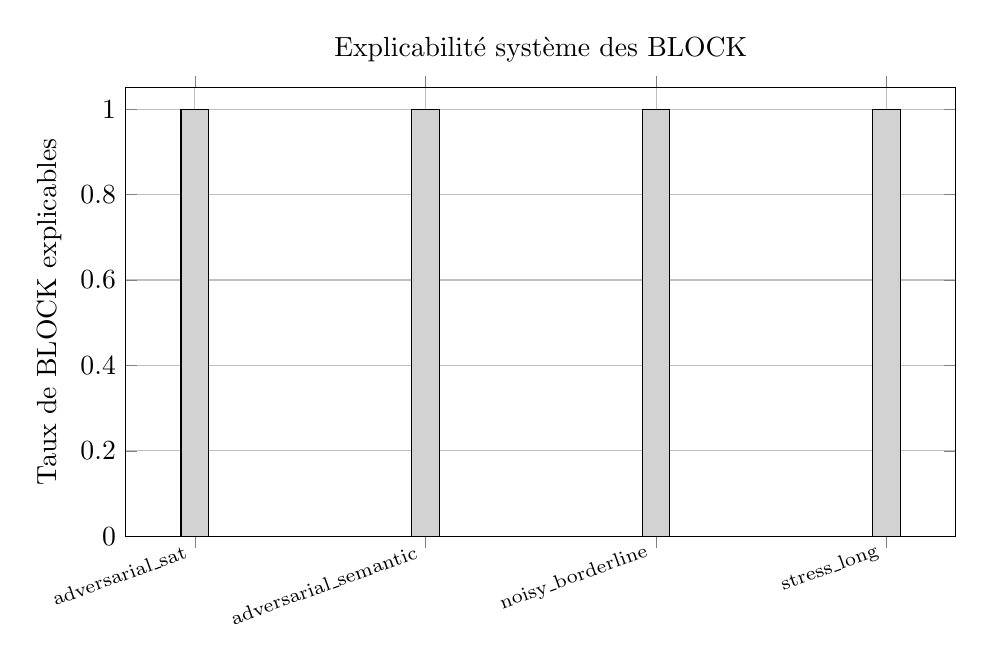
\begin{tikzpicture}
\begin{axis}[ybar,
bar width=10pt,
width=\linewidth,
height=0.60\linewidth,
title={Explicabilité système des BLOCK},
ylabel={Taux de BLOCK explicables},
xtick={0,1,2,3},
xticklabels={{adversarial\_sat},{adversarial\_semantic},{noisy\_borderline},{stress\_long}},
x tick label style={rotate=20,anchor=east,font=\scriptsize},
ymin=0,
grid=major,
ymax=1.05]
\addplot+[draw=black,fill=gray!35] coordinates {(0,1.0) (1,1.0) (2,1.0) (3,1.0)};
\end{axis}
\end{tikzpicture}
